\chapter[Hardware-Software Codesign]{Hardware/Software Codesign}\label{ch:fpga-codesign}
\openepigraph{Because of the nature of Moore's law, anything that an extremely clever graphics programmer can do at one point can be replicated by a merely competent programmer some number of years later.}{John Carmack}
The process of achieving desired functionality on a system by exploring a design space and mapping tasks to resources within system constraints is referred to as Hardware/Software Codesign~\cite{6172642}. 
\newthoughtpar{Implementing Neural Networks on FPGAs}
To aid our understanding of how a neural network is optimized for inference on an FPGA, we glance at the HLS-RFNoC workflow. This is an open source workflow for deploying a neural network for inference on an FPGA for RF signal processing~\cite{Charles2013}. This implementation uses Vivado HLS to generate custom HDL for the neural network. HLS4ML~\cite{nhan_tran_2019_3359214} is used to create the neural-network C++ code used with Vivado HLS. 
The steps can be summarized as below:
\begin{itemize}
    \item Prototype and train a neural network with industry standard machine learning framework.
    \item Use the HLS4ML C++ generation tool to create a starting point for running Xilinx HLS.
    \item Synthesize the HLS to evaluate resource usage. Once the network is implemented in fixed-point, run HLS synthesis to create HDL code.
    \item Module resulting from HDL generation is inserted into an RFNoC Compute Engine. A user testbench is then optionally created to stimulate the CE and validate its functionality. 
    \item The Compute Engine is then built into an FPGA Image using the RFNoC image building workflow.
\end{itemize}

There are some key abstractions that may make generating an efficient run-time strategy difficult. The first being, there is no insight into how a specific prototype topology would map to an FPGA in terms of cost. The entry point for most FPGA vendor tools are Register Transfer Level (RTL) designs, expressed in VERILOG or VHDL~\cite{umuroglu2018accelerating}. This brings about the second, the compiler is responsible for translating the neural network into the language of the instruction set, scheduling memory transfers on the target hardware. In the next chapter, we will further discuss how these problems manifest negatively in hardware/software codesign and discuss our proposed design methodology. 


\begin{table}
    \begin{sidecaption}[Static Mapping Cost]{%
        Static Mapping Cost to 6:1 LUTs for Fan-In bits.
    }[st:tab:staticlutcost]
    \centering
    \begin{threeparttable}
    \renewcommand{\arraystretch}{1.2}
    \begin{tabular}{lrrrr}
        \toprule 
        Fan-In & Number of 6-LUTs & Truth table bits & LUT config bits & \% utilized \\  \midrule

        6 \            &  1  & 64   &     64   & 100\%    \\ 
        7\             &  3  & 128  &     192  & 66.67\%  \\ 
        8\             &  5  & 256  &     320  & 80\%     \\ 
        9\             &  11 & 512  &     704  & 72.73\%  \\ 
        10 \           &  21 & 1024 &     1344 & 76.19\%  \\ 
        11\            &  43 & 2048 &     2752 & 74.42\%  \\ 
        \bottomrule
    \end{tabular}
    \end{threeparttable}
    \end{sidecaption}
\end{table}

\section{Fan-in, Neurons and LUTs.}
One of the central concepts we must grasp to be able to delve into how we can effectively generate topologies in a Machine Learning framework which effectively map to FPGAs is how a Neuron with specific total Fan-In bits and output bits are mapped to LUTs. A brief mapping cost has been detailed in \cref{st:tab:staticlutcost}.
We deal with the mathematics behind it and attempt to give the reader a visual understanding of how the process is carried out.

\newthoughtpar{Mapping to 6:1 LUTs}
\cref{fig:71lutto61luts} and \cref{fig:81lutto61luts} depict how we can map a 7:1 and 8:1 Truth Table to 6:1 LUTs respectively. We can extend similarly to larger input-output bit configurations, which is being discussed below in more detail.

\marginpar{\centering
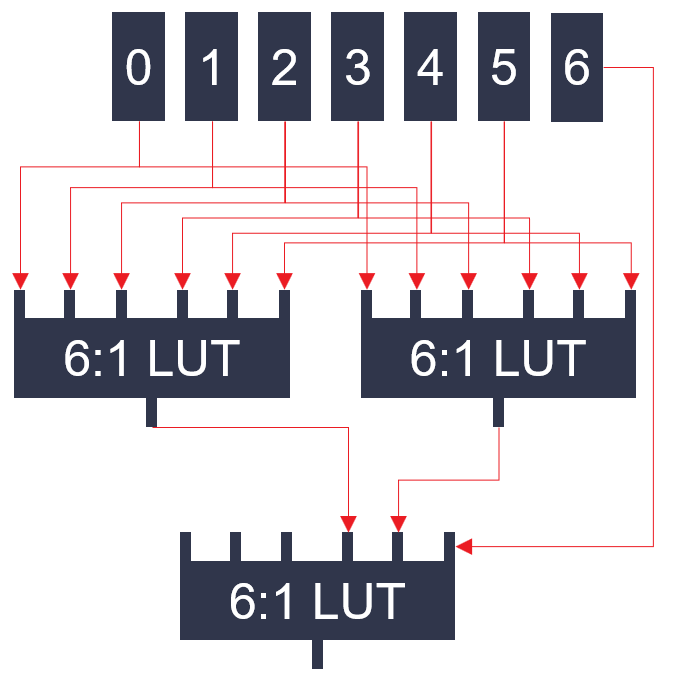
\includegraphics[width=130pt]{figures/bison/71lutw61luts.png}
\captionof{figure}{Mapping a 7:1 Look-up Table to 6:1 LUTs.}
\label{fig:71lutto61luts}
% \endgroup
}
\marginpar{\centering
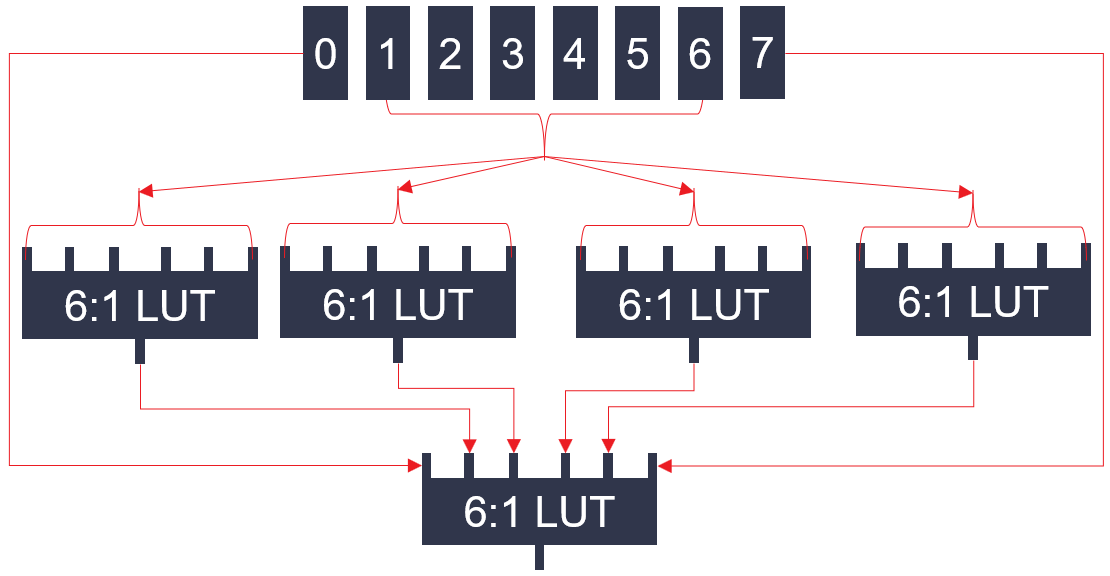
\includegraphics[width=130pt]{figures/bison/81lutw61luts.png}
\captionof{figure}{Mapping a 8:1 Look-up Table to 6:1 LUTs.}
\label{fig:81lutto61luts}
% \endgroup
}

\newthoughtpar{Closed Form equation for LUT cost.}
We attempt to develop a Closed Form equation for the theoretical LUT cost of implementing a specific Neuron with arbitrary Fan-in and Fan-out.
The recursive form of the equation for the LUT cost of a neuron with $N$ fan-in bits and $M$ output bits is given by \eqref{recursiveform1}
\begin{equation}
    LUT_{N, M} = M\times(2\times(\frac{LUT_{N-1, M}}{M}) - (-1)^{N})
    \label{recursiveform1}
\end{equation}

This can be further simplified to \eqref{recursiveform2}. 
\begin{equation}
    LUT_{N, M} = M\times(\frac{LUT_{N-2, M}}{M} + 2^{N-6})
    \label{recursiveform2}
\end{equation}

Which in its closed form gives us \eqref{lutcostcloseform}. Note that these LUT costs will only be valid for hardware building blocks composed solely from 6:1 LUTs. Getting the minimum LUT cost from the combination of the wide array of memory types that an FPGA has (5:2 LUTs, 6:1 LUTs, different BRAM configurations) is a design space exploration problem. This elementary equation is integrated into the design flow to give the user a rough hardware cost heuristic. There are many ways to decrease this cost, which will be discussed later.
\begin{equation}
    LUT_{N, M} = M\times(\frac{2^{N-4} - (-1)^{N}}{3})
    \label{lutcostcloseform}
\end{equation}




% /*
% Introduction
% The need for accelerators
%     CPUs, GPUs, ASICs, FPGAs.
% Background
%     FPGA and HW/SW Co-Design
%     Mapping Neurons to Hardware
%       Sparsity
%           Expander, Iterative, Momentum
%       Quantize
%           Activation brevitas
%           Non Linear
% FPGANet: A Library for Mapping HBBs to NEQs
%     Introduction
%     Components
%       Linear
%       Convolutions
%     Design Automation
%       TruthTableGen
%       VerilogGen
%       Synthesis
% Testing FPGANet
%     FPGANet4HEP
%       Introduction
%       Models
%     MNIST 
%       Models
% Concluding Remarks
%     Research Questions
%     Conclusion
% */